\documentclass[12pt,a4paper]{report}
\usepackage[italian]{babel}
\usepackage{newlfont}
\usepackage{ragged2e}
\usepackage{csquotes}
\usepackage{hyperref, cleveref}
\usepackage{graphicx, caption, subcaption}

%Bibliografia
\usepackage[style=numeric,sorting=none]{biblatex}
\addbibresource{bibliografia.bib}

\textwidth=450pt\oddsidemargin=0pt

\begin{document}
\begin{titlepage}

\begin{center}
{{\Large{\textsc{Alma Mater Studiorum $\cdot$ Universit\`a di Bologna}}}} 
\rule[0.1cm]{15.8cm}{0.1mm}
\rule[0.5cm]{15.8cm}{0.6mm}
\\\vspace{3mm}

{\small{\bf Scuola di Scienze \\ 
Dipartimento di Fisica e Astronomia\\
Corso di Laurea in Fisica}}

\end{center}

\vspace{23mm}

\begin{center}\
{\LARGE{\bf Redazione della voce dell'enciclopedia online Wikipedia riguardante la Spettroscopia}}\\
\end{center}

\vspace{50mm} \par \noindent

\begin{minipage}[t]{0.47\textwidth}\raggedright 
{\large{\bf Relatore: \vspace{2mm}\\
Prof. Enrico Gianfranco Campari
}}
\end{minipage}
%
\hfill
%
\begin{minipage}[t]{0.47\textwidth}\raggedleft
{\large{\bf Presentata da:
\vspace{2mm}\\
Riccardo Peltretti}}
\end{minipage}

\vspace{40mm}

\begin{center}
Anno Accademico 2023/2024
\end{center}

\end{titlepage}

\vspace*{\fill}
\begin{flushright}
It is a good thing for an uneducated man to read books of quotations
\end{flushright}
\vspace*{\fill}\newpage

\tableofcontents
\newpage

\chapter{Wikipedia: stora e impatto sulla divulgazione}

\section{Introduzione a Wikipedia}

Wikipedia è un'enciclopedia online gratuita, collaborativa e multilingue, fondata il 15 gennaio 2001 da Jimmy Wales e Larry Sanger \cite{lih2009wikipedia}. Il nome è una combinazione del termine "wiki", che indica un tipo di sito web che permette la creazione e modifica collaborativa dei contenuti, e "encyclopedia", dal greco "paideia" che significa educazione o cultura generale. Il termine "wiki", a sua volta, deriva dalla parola hawaiana "wikiwiki", che significa "veloce" o "rapido". Questa scelta rifletteva l'obiettivo di creare un'enciclopedia che potesse essere rapidamente modificata e aggiornata da chiunque avesse accesso a Internet \cite{cunningham2001wiki}. 

Il primo software wiki, chiamato WikiWikiWeb, fu sviluppato da Ward Cunningham nel 1995 per facilitare la condivisione e l'organizzazione collaborativa delle informazioni \cite{cunningham2001wiki}. Wikipedia sfrutta questo modello per consentire agli utenti di creare e modificare le voci tramite un'interfaccia semplice e intuitiva. Gli utenti possono creare nuove pagine, aggiornare quelle esistenti e correggere errori, mantenendo un vasto database di conoscenze. La piattaforma è accessibile a chiunque abbia una connessione Internet e, sebbene non sia necessario registrarsi per consultare le voci, creare un account offre ulteriori vantaggi e funzionalità.

Le voci di Wikipedia sono organizzate in modo ipertestuale, con numerosi link interni che connettono argomenti correlati. Questa struttura facilita la navigazione e permette ai lettori di esplorare un argomento in profondità. Ogni pagina contiene una sezione di riferimento che elenca le fonti utilizzate, garantendo la verificabilità delle informazioni \cite{denning2005wikipedia}.

Wikipedia è mantenuta da una vasta comunità di volontari, noti come Wikipediani, che contribuiscono alla creazione, revisione e manutenzione delle voci. Ci sono diverse categorie di utenti con ruoli specifici, come gli amministratori, che hanno accesso a strumenti avanzati per la gestione del sito, e i revisori, che controllano la qualità dei contenuti. Le modifiche alle voci sono monitorate tramite una cronologia delle revisioni, che registra ogni cambiamento e permette di ripristinare versioni precedenti in caso di errori o vandalismi. Inoltre, le pagine di discussione permettono agli utenti di confrontarsi su come migliorare le voci \cite{reagle2010good}.

\subsection{Principi e obiettivi}

Wikipedia opera secondo una serie di principi fondamentali che ne guidano il funzionamento e ne assicurano l'integrità e la qualità delle informazioni. Questi principi includono la neutralità, la verificabilità e il contenuto libero.

Il principio di neutralità (NPOV - Neutral Point Of View) richiede che tutte le voci siano scritte in modo imparziale, presentando i fatti senza pregiudizi e riflettendo equamente i diversi punti di vista su un argomento \cite{reagle2010good}. La verificabilità è un altro principio cruciale: ogni informazione deve essere supportata da fonti affidabili che possono essere controllate dai lettori \cite{denning2005wikipedia}. Questo richiede che gli editori citino fonti come libri accademici, articoli scientifici e pubblicazioni giornalistiche, per garantire che i contenuti siano basati su prove concrete.

Tutti i testi e i media pubblicati su Wikipedia sono disponibili sotto licenze libere, come la Creative Commons Attribution-ShareAlike License (CC BY-SA). Questo principio permette a chiunque di utilizzare, modificare e distribuire i contenuti di Wikipedia, purché venga data attribuzione agli autori originali e le opere derivate siano distribuite con la stessa licenza \cite{jemielniak2014wikipedia}.

Gli utenti di Wikipedia devono seguire una serie di linee guida editoriali che aiutano a mantenere la coerenza e la qualità delle voci, includendo la citazione delle fonti, l'evitare conflitti di interesse e il rispetto delle politiche di copyright. Le voci devono essere scritte in modo chiaro e comprensibile, evitando l'uso di linguaggio tecnico non necessario \cite{reagle2010good}.

Wikipedia si impegna a migliorare continuamente la sua piattaforma e i suoi contenuti. Questo include l'aggiornamento delle tecnologie utilizzate, l'introduzione di nuove funzionalità per facilitare la collaborazione e la modifica dei contenuti, e l'implementazione di strumenti per migliorare la qualità delle voci \cite{history_of_wikis}.

\subsection{Struttura e funzionamento generale}

Wikipedia utilizza il software MediaWiki, sviluppato appositamente per Wikipedia e altre iniziative del movimento Wikimedia \cite{denning2005wikipedia}. MediaWiki è un potente software open source che offre numerose funzionalità avanzate per la gestione dei contenuti, il controllo delle versioni e la collaborazione in tempo reale.

Gli utenti possono contribuire anonimamente o creare un account per ottenere ulteriori funzionalità, come la possibilità di tenere traccia delle modifiche effettuate e discutere con altri utenti. Ogni pagina di Wikipedia dispone di una cronologia delle modifiche, che registra tutte le versioni precedenti della pagina, consentendo agli utenti di ripristinare versioni precedenti in caso di vandalismo o errori \cite{wikiwikiweb}. Inoltre, le pagine di discussione associate a ciascuna voce consentono agli utenti di confrontarsi sulle modifiche da apportare, promuovendo un ambiente di collaborazione e miglioramento continuo \cite{jemielniak2014wikipedia}.

Ogni pagina contiene anche una sezione di riferimento che elenca le fonti utilizzate, garantendo la verificabilità delle informazioni. La struttura ipertestuale e la facilità di navigazione sono elementi chiave che contribuiscono all'efficacia di Wikipedia come risorsa educativa \cite{reagle2010good}.

Wikipedia adotta un modello di gestione decentralizzato, in cui la comunità degli utenti svolge un ruolo cruciale nel mantenimento e nella qualità delle voci. Gli amministratori, eletti dalla comunità, hanno accesso a strumenti avanzati per la gestione del sito e per la risoluzione delle dispute. Essi possono bloccare utenti problematici, proteggere pagine sensibili e intervenire nei conflitti editoriali \cite{denning2005wikipedia}.

Inoltre, Wikipedia utilizza una serie di bot, ovvero programmi automatizzati, per eseguire compiti ripetitivi come il controllo dei link interrotti, la rimozione di spam e l'aggiornamento delle informazioni. Questi bot contribuiscono a mantenere l'enciclopedia in ordine e a garantire che le informazioni siano sempre aggiornate \cite{history_of_wikis}.

In sintesi, la struttura e il funzionamento generale di Wikipedia si basano su un software avanzato e su una comunità collaborativa, supportata da un sistema di controllo delle modifiche e da strumenti automatizzati che garantiscono la qualità e l'affidabilità delle informazioni.

\subsection{I cinque pilastri di Wikipedia}

I cinque pilastri di Wikipedia costituiscono i principi fondamentali che guidano il funzionamento e la gestione dell'enciclopedia. Questi pilastri sono stati concepiti per mantenere l'integrità, la qualità e la neutralità dei contenuti, garantendo che Wikipedia rimanga una risorsa affidabile e accessibile a tutti. Essi sono:

\paragraph*{1. Wikipedia è un'enciclopedia}
Il primo pilastro stabilisce che Wikipedia è, prima di tutto, un'enciclopedia. Ciò significa che il suo scopo principale è raccogliere e presentare informazioni in modo accurato e verificabile. Wikipedia non è una raccolta indiscriminata di informazioni, un luogo per la promozione personale, una piattaforma di propaganda, o un forum di discussione. Le voci devono essere basate su fonti attendibili e riflettere la conoscenza consolidata, evitando ricerche originali \cite{reagle2010good}.

\paragraph*{2. Wikipedia ha un punto di vista neutrale}
Il secondo pilastro impone che le voci di Wikipedia siano scritte da un punto di vista neutrale (NPOV - Neutral Point Of View). Questo implica che le informazioni devono essere presentate in modo imparziale, rappresentando tutti i punti di vista rilevanti in maniera equa e proporzionata. Gli editori devono evitare di inserire opinioni personali e devono basare le loro affermazioni su fonti verificabili. La neutralità è essenziale per mantenere la credibilità di Wikipedia come fonte di informazione \cite{denning2005wikipedia}.

\paragraph*{3. Wikipedia è libera}
Il terzo pilastro stabilisce che tutto il contenuto di Wikipedia è libero e gratuito. Le voci sono pubblicate sotto licenze libere, come la Creative Commons Attribution-ShareAlike License (CC BY-SA), che permette a chiunque di usare, modificare e distribuire i contenuti, a condizione che venga data attribuzione agli autori originali e che le opere derivate siano rilasciate sotto la stessa licenza \cite{jemielniak2014wikipedia}. Questo principio promuove la diffusione della conoscenza e la collaborazione aperta.

\paragraph*{4. Wikipedia ha un codice di condotta}
Il quarto pilastro riguarda il comportamento degli utenti. Wikipedia incoraggia un ambiente di rispetto e collaborazione. Gli editori devono agire con cortesia e civiltà, evitando attacchi personali e rispettando le opinioni degli altri. Le discussioni sulle modifiche delle voci devono essere condotte in modo costruttivo e rispettoso, facilitando la risoluzione delle dispute e la collaborazione efficace \cite{history_of_wikis}.

\paragraph*{5. Wikipedia non ha regole fisse}
Il quinto pilastro stabilisce che Wikipedia non ha regole fisse oltre i cinque pilastri stessi. Le linee guida e le politiche possono evolvere con il tempo per adattarsi alle nuove esigenze della comunità e del progetto. La flessibilità è fondamentale per permettere a Wikipedia di crescere e migliorare continuamente. Gli utenti sono incoraggiati a essere audaci nelle modifiche, ma sempre con la consapevolezza di rispettare i principi fondamentali \cite{reagle2010good}.

I cinque pilastri di Wikipedia costituiscono la base della sua filosofia e delle sue operazioni. Essi garantiscono che Wikipedia rimanga una risorsa libera, neutrale e collaborativa, impegnata nella diffusione della conoscenza in tutto il mondo.

\section{Storia di Wikipedia}

\subsection{Le origini e la fondazione (2001)}

Wikipedia è stata fondata il 15 gennaio 2001 da Jimmy Wales e Larry Sanger. L'idea di creare un'enciclopedia online libera e collaborativa nacque dal progetto Nupedia, un'enciclopedia online scritta da esperti e revisionata in modo rigoroso. Nupedia, fondata da Jimmy Wales, era un progetto ambizioso ma soffriva di lentezza nel processo di revisione, che limitava la velocità di ampliamento del contenuto \cite{lih2009wikipedia}.

Per superare questi limiti, Larry Sanger, che lavorava come redattore capo di Nupedia, propose di utilizzare un modello wiki per accelerare il processo di creazione e revisione delle voci. Permettendo agli utenti di collaborare direttamente nella stesura delle voci, con la possibilità di correggere e migliorare continuamente i contenuti, wikipedia fu messa nelle condizioni di sostenere una crescita organica vigorosa\cite{reagle2010good}.

Il 15 gennaio 2001, Wikipedia fu lanciata ufficialmente come un progetto complementare a Nupedia. Inizialmente, Wikipedia era vista come un esperimento per supportare Nupedia, ma presto dimostrò di avere un potenziale molto maggiore. Grazie alla sua natura aperta e collaborativa, Wikipedia crebbe rapidamente, attirando contributi da parte di utenti di tutto il mondo. Entro il primo anno, Wikipedia aveva già raccolto migliaia di voci in diverse lingue \cite{jemielniak2014wikipedia}.

La filosofia alla base di Wikipedia era quella di creare una risorsa di conoscenza libera e accessibile a tutti, basata sui principi di neutralità, verificabilità e contenuto libero. Questo approccio democratizzava l'accesso alla conoscenza e permetteva la creazione di contenuti in modo collaborativo, sfruttando l'intelligenza collettiva della comunità globale \cite{denning2005wikipedia}.

La nascita di Wikipedia rappresentò un momento cruciale nella storia della diffusione della conoscenza. Da un esperimento nato per supportare Nupedia, Wikipedia si trasformò rapidamente in uno dei principali punti di riferimento per l'informazione online, grazie alla sua natura aperta e collaborativa.

\subsection{Evoluzione e crescita nel tempo}

Dalla sua fondazione nel 2001, Wikipedia ha conosciuto una crescita esponenziale, figura \cref{fig:wikiPagesYear}, diventando una delle principali fonti di informazione su Internet. Nei primi anni, il progetto attirò rapidamente l'attenzione di utenti di tutto il mondo, grazie alla sua natura aperta e collaborativa che permetteva a chiunque di contribuire al contenuto dell'enciclopedia \cite{lih2009wikipedia}.

Nel 2003, fu creata la Wikimedia Foundation, un'organizzazione senza scopo di lucro, per supportare Wikipedia e i suoi progetti correlati. La fondazione si occupa della raccolta di fondi, del supporto tecnico e della promozione della missione di Wikipedia di fornire contenuti liberi e accessibili a tutti \cite{reagle2010good}. La creazione della Wikimedia Foundation ha permesso a Wikipedia di ottenere maggiore stabilità e risorse per continuare a crescere.

Nel corso degli anni, Wikipedia ha introdotto numerose funzionalità e miglioramenti tecnici. Ad esempio, nel 2004 fu implementato il sistema di categorie, che permette di organizzare le voci in gruppi tematici, facilitando la navigazione e la ricerca delle informazioni \cite{jemielniak2014wikipedia}. Nel 2007, fu lanciato il VisualEditor, uno strumento che consente agli utenti di modificare le voci utilizzando un'interfaccia WYSIWYG (What You See Is What You Get), rendendo più semplice la partecipazione anche per coloro che non hanno familiarità con il markup wiki \cite{history_of_wikis}.

La comunità di Wikipedia ha continuato a crescere, con un numero sempre maggiore di utenti che contribuiscono al miglioramento e all'espansione delle voci. La partecipazione attiva della comunità è uno degli elementi chiave del successo di Wikipedia, poiché permette una revisione continua e collaborativa dei contenuti. Gli utenti possono discutere sulle modifiche da apportare alle voci nelle pagine di discussione, promuovendo un ambiente di collaborazione e miglioramento continuo \cite{denning2005wikipedia}.

\begin{figure}
    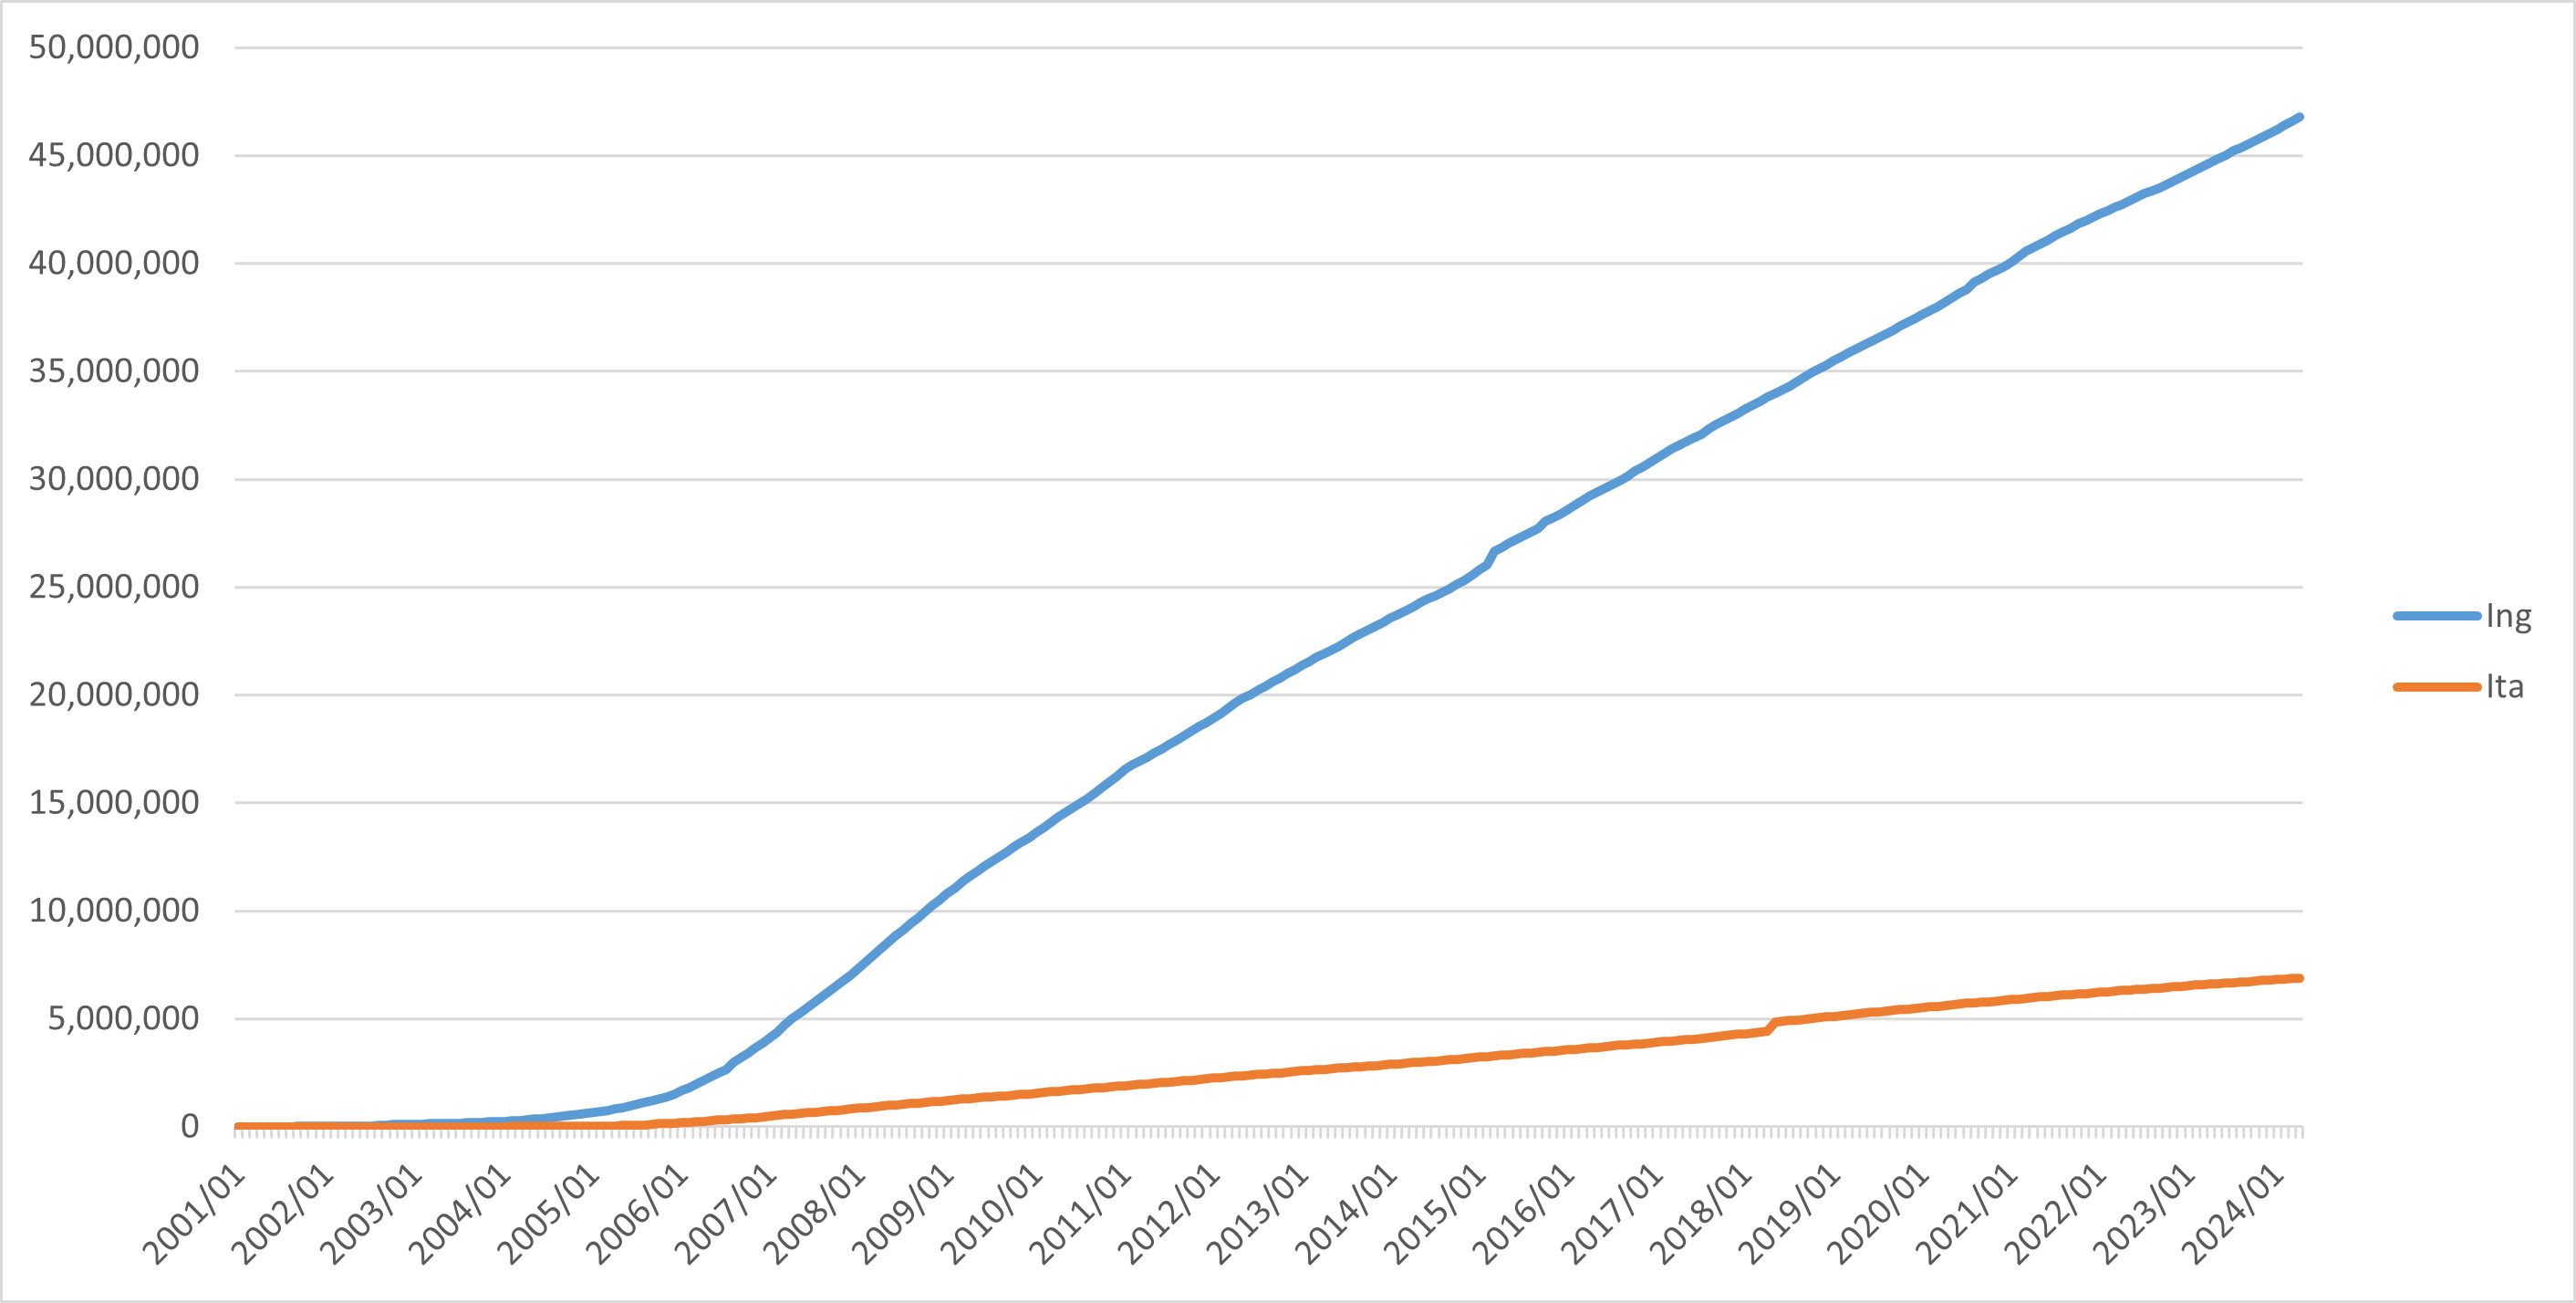
\includegraphics[width=\linewidth]{Immagini/Grafico pagine wikipedia excel.png}
    \caption{Numero complessivo di pagine di Wikipedia in lingua inglese e italiana in riferimento all'anno, dal 2001 ad oggi.\cite{wikimedia_stats} }
    \captionsetup{width=.8\linewidth}
    \label{fig:wikiPagesYear}
\end{figure}

Wikipedia è diventata disponibile in un numero crescente di lingue, riflettendo la sua missione di rendere la conoscenza accessibile a livello globale. Attualmente, Wikipedia esiste in oltre 300 lingue, con milioni di voci che coprono una vasta gamma di argomenti. Le edizioni in lingue diverse dall'inglese continuano a crescere, contribuendo a rendere Wikipedia una risorsa veramente globale \cite{reagle2010good}.

Nel corso degli anni, Wikipedia ha affrontato e superato numerose sfide, tra cui problemi di vandalismo, questioni di qualità delle informazioni e critiche sulla sua affidabilità. Per affrontare questi problemi, la comunità di Wikipedia ha sviluppato una serie di politiche e linee guida, come il controllo delle modifiche e l'adozione di strumenti automatizzati (bot) per monitorare e migliorare la qualità dei contenuti \cite{jemielniak2014wikipedia}.

Grazie a questi sforzi, Wikipedia è diventata una delle risorse più consultate al mondo, utilizzata quotidianamente da milioni di persone per ottenere informazioni su una vasta gamma di argomenti. La sua evoluzione e crescita nel tempo dimostrano il potere della collaborazione aperta e della condivisione della conoscenza.

\subsection{Milestones e sviluppi significativi}

Nel 2003, la creazione della Wikimedia Foundation rappresentò un importante passo avanti per Wikipedia. La fondazione, una organizzazione senza scopo di lucro, fu istituita per fornire supporto tecnico, legale e finanziario al progetto. Questo ha permesso a Wikipedia di crescere in modo sostenibile e di mantenere la sua indipendenza editoriale \cite{reagle2010good}.

Nel 2004, fu introdotto il sistema di categorie, che ha migliorato notevolmente l'organizzazione e la navigazione delle voci su Wikipedia. Questo sistema permette di raggruppare le voci in base a temi comuni, facilitando la ricerca delle informazioni e la scoperta di contenuti correlati \cite{jemielniak2014wikipedia}.

Un'altra importante milestone fu l'introduzione del VisualEditor nel 2013. Questo strumento ha rivoluzionato il modo in cui gli utenti possono modificare le voci, offrendo un'interfaccia WYSIWYG (What You See Is What You Get) che semplifica l'editing anche per coloro che non hanno familiarità con il markup wiki \cite{history_of_wikis}. Il VisualEditor ha reso la modifica delle pagine più accessibile, incoraggiando una partecipazione più ampia.

Nel corso degli anni, Wikipedia ha implementato vari strumenti di controllo della qualità e meccanismi di revisione. Tra questi, il sistema di "flagged revisions", introdotto nel 2008, che permette a determinati utenti di revisionare e approvare modifiche prima che queste diventino visibili al pubblico. Questo ha contribuito a migliorare la qualità e l'affidabilità delle informazioni presenti su Wikipedia \cite{denning2005wikipedia}.

Un'importante evoluzione nella gestione dei contenuti è stata l'integrazione con Wikidata nel 2012. Wikidata è un database collaborativo che fornisce dati strutturati per supportare Wikipedia e altri progetti della Wikimedia Foundation. Questa integrazione ha permesso di migliorare la coerenza e l'aggiornamento delle informazioni tra le varie versioni linguistiche di Wikipedia \cite{history_of_wikis}.

Wikipedia ha anche affrontato sfide legali e di censura in diversi paesi. Ad esempio, nel 2010, Wikipedia fu temporaneamente bloccata in Cina a causa di contenuti considerati sensibili dal governo cinese. La comunità di Wikipedia e la Wikimedia Foundation hanno lavorato costantemente per affrontare queste sfide, cercando di garantire l'accesso libero all'informazione per tutti \cite{jemielniak2014wikipedia}.

Nel 2021, Wikipedia ha celebrato il suo 20º anniversario, un traguardo significativo che ha evidenziato il suo ruolo cruciale nella diffusione della conoscenza libera. Con milioni di voci in centinaia di lingue, Wikipedia continua a crescere e a evolversi, mantenendo il suo impegno verso la neutralità, la verificabilità e il contenuto libero \cite{reagle2010good}.

\section{Impatto sulla divulgazione scientifica e culturale}

\subsection{Wikipedia come risorsa educativa}

Wikipedia è ampiamente riconosciuta come una risorsa educativa preziosa, utilizzata da studenti, insegnanti e ricercatori di tutto il mondo. La sua accessibilità gratuita e la vastità delle informazioni disponibili la rendono uno strumento ideale per l'apprendimento autodiretto e la ricerca preliminare \cite{reagle2010good}.

Gli studenti utilizzano frequentemente Wikipedia come punto di partenza per le loro ricerche. Le voci di Wikipedia forniscono panoramiche generali sugli argomenti, complete di riferimenti a fonti esterne che possono essere consultate per un approfondimento ulteriore. Questa caratteristica aiuta gli studenti a comprendere rapidamente i concetti di base e a identificare le risorse accademiche rilevanti \cite{denning2005wikipedia}.

Gli insegnanti trovano in Wikipedia uno strumento utile per integrare le loro lezioni. Possono utilizzare le voci di Wikipedia per assegnare letture agli studenti, sviluppare materiali didattici e stimolare discussioni in classe. Inoltre, Wikipedia offre una piattaforma per progetti educativi in cui gli studenti possono contribuire alla creazione e alla modifica delle voci, sviluppando così competenze di ricerca, scrittura e pensiero critico \cite{jemielniak2014wikipedia}.

Uno degli aspetti più significativi di Wikipedia come risorsa educativa è la sua capacità di promuovere l'alfabetizzazione digitale. Utilizzando Wikipedia, gli studenti imparano a valutare criticamente le informazioni, a distinguere tra fonti affidabili e non affidabili e a comprendere l'importanza della citazione delle fonti. Queste competenze sono essenziali in un'epoca in cui l'accesso alle informazioni è vasto e spesso caotico \cite{lih2009wikipedia}.

Wikipedia è anche uno strumento potente per la promozione dell'apprendimento continuo. Gli utenti di tutte le età possono utilizzare l'enciclopedia per esplorare nuovi interessi, approfondire conoscenze esistenti e rimanere aggiornati su una vasta gamma di argomenti. La natura collaborativa di Wikipedia permette agli utenti di condividere il loro sapere e di apprendere dagli altri, creando una comunità globale di apprendimento \cite{history_of_wikis}.

Le collaborazioni tra Wikipedia e istituzioni educative hanno portato a numerosi progetti di successo. Ad esempio, il programma Wikipedia Education Program coinvolge studenti e docenti in tutto il mondo, incoraggiandoli a contribuire a Wikipedia come parte del loro percorso accademico. Questi progetti non solo arricchiscono il contenuto di Wikipedia, ma forniscono anche agli studenti un'esperienza pratica nella ricerca e nella scrittura accademica \cite{jemielniak2014wikipedia}.

Nonostante le sue numerose qualità, Wikipedia affronta anche critiche come risorsa educativa. Alcuni educatori esprimono preoccupazioni riguardo alla qualità e all'affidabilità delle informazioni presenti su Wikipedia. Tuttavia, la comunità di Wikipedia e la Wikimedia Foundation lavorano costantemente per migliorare la qualità delle voci attraverso politiche di revisione, l'uso di fonti affidabili e l'integrazione di strumenti automatizzati per il controllo delle modifiche \cite{denning2005wikipedia}.

In conclusione, Wikipedia rappresenta una risorsa educativa versatile e potente, capace di supportare l'apprendimento in molti modi. La sua accessibilità, la vastità dei contenuti e la capacità di promuovere l'alfabetizzazione digitale la rendono uno strumento indispensabile nell'educazione moderna.

\subsection{La qualità e l'affidabilità delle informazioni}

La qualità e l'affidabilità delle informazioni su Wikipedia sono temi di fondamentale importanza, sia per la comunità degli utenti che per i lettori. Essendo un'enciclopedia aperta e collaborativa, Wikipedia deve affrontare la sfida di mantenere standard elevati di accuratezza e affidabilità nonostante la possibilità di modifiche da parte di chiunque \cite{reagle2010good}.

Un elemento chiave per garantire la qualità delle informazioni è il principio di verificabilità. Ogni informazione presente su Wikipedia deve essere supportata da fonti affidabili che possono essere controllate dai lettori. Questo principio richiede che gli editori citino fonti autorevoli, come libri accademici, articoli scientifici e pubblicazioni giornalistiche, per garantire che i contenuti siano basati su prove concrete e verificabili \cite{denning2005wikipedia}.

Wikipedia adotta una politica di neutralità, il che significa che le voci devono essere scritte in modo imparziale, presentando i fatti senza pregiudizi. Questo è essenziale per mantenere la credibilità dell'enciclopedia e per garantire che le informazioni fornite siano equilibrate e rappresentative dei diversi punti di vista su un argomento \cite{reagle2010good}.

Wikipedia utilizza anche bot, ovvero programmi automatizzati, per eseguire compiti ripetitivi come il controllo dei link interrotti, la rimozione di spam e l'aggiornamento delle informazioni. Questi bot contribuiscono a mantenere l'enciclopedia in ordine e a garantire che le informazioni siano sempre aggiornate e accurate \cite{history_of_wikis}.

Le politiche editoriali di Wikipedia richiedono che le voci siano scritte in un linguaggio chiaro e comprensibile, evitando l'uso di linguaggio tecnico non necessario. Questo aiuta a rendere le informazioni accessibili a un pubblico ampio e diversificato, migliorando la comprensione e l'usabilità delle voci \cite{reagle2010good}.

Nonostante queste misure, Wikipedia affronta critiche riguardo alla qualità e all'affidabilità delle informazioni. Alcuni studiosi e professionisti esprimono preoccupazioni sul fatto che l'apertura della piattaforma possa portare a errori e informazioni fuorvianti. Tuttavia, studi comparativi hanno dimostrato che, in molti casi, la qualità delle informazioni su Wikipedia è paragonabile a quella delle enciclopedie tradizionali, come l'Enciclopedia Britannica \cite{giles2005nature}.

Per affrontare queste critiche, la comunità di Wikipedia continua a sviluppare e migliorare le politiche di revisione e controllo della qualità. Questo include l'implementazione di strumenti avanzati per l'analisi delle modifiche, la formazione di gruppi di lavoro specializzati e la collaborazione con esperti in vari campi del sapere. Questi sforzi collettivi aiutano a mantenere Wikipedia come una risorsa affidabile e rispettabile per milioni di utenti in tutto il mondo \cite{jemielniak2014wikipedia}.

\subsection{Contributi alla scienza e alla conoscenza pubblica}

Wikipedia ha avuto un impatto significativo sulla scienza e sulla conoscenza pubblica, fungendo da ponte tra il pubblico generale e la comunità scientifica. Essendo una delle risorse online più consultate al mondo, Wikipedia rende le informazioni scientifiche accessibili a milioni di persone, promuovendo una maggiore comprensione di argomenti complessi \cite{reagle2010good}.

Uno dei principali contributi di Wikipedia è la democratizzazione dell'accesso alla conoscenza. Prima dell'avvento di Wikipedia, l'accesso a informazioni di qualità era spesso limitato a coloro che potevano permettersi costose enciclopedie o iscrizioni a riviste accademiche. Wikipedia ha eliminato queste barriere, rendendo la conoscenza disponibile gratuitamente a chiunque abbia una connessione Internet \cite{lih2009wikipedia}.

Wikipedia svolge un ruolo cruciale nella diffusione delle scoperte scientifiche. Gli articoli su Wikipedia vengono frequentemente aggiornati per riflettere le ultime ricerche e scoperte, rendendo possibile per il pubblico rimanere informato sugli sviluppi più recenti in vari campi della scienza. Questo è particolarmente evidente nelle voci riguardanti la medicina, la fisica, la biologia e le scienze ambientali \cite{jemielniak2014wikipedia}.

La piattaforma è utilizzata anche come strumento educativo nelle università e nelle scuole. Molti docenti incoraggiano gli studenti a utilizzare Wikipedia come punto di partenza per le loro ricerche, grazie alla sua capacità di fornire panoramiche generali e riferimenti a fonti più dettagliate. Inoltre, diversi programmi educativi coinvolgono gli studenti nella creazione e nella modifica delle voci di Wikipedia, fornendo loro un'esperienza pratica nella ricerca e nella scrittura accademica \cite{denning2005wikipedia}.

Un ulteriore contributo di Wikipedia alla qualità e all'affidabilità delle informazioni risiede nel suo sostegno alla scienza aperta (open science). La scienza aperta promuove la trasparenza, la condivisione dei dati e la collaborazione tra ricercatori di tutto il mondo. Wikipedia, con il suo modello aperto e collaborativo, incarna molti dei principi della scienza aperta, rendendo le informazioni scientifiche accessibili a chiunque. Le voci scientifiche di Wikipedia spesso includono riferimenti a ricerche e dati disponibili liberamente, incoraggiando la condivisione del sapere e il coinvolgimento della comunità scientifica e del pubblico generale. Questo approccio non solo aumenta la trasparenza, ma facilita anche la verifica delle informazioni e la replicazione degli studi, elementi fondamentali per il progresso scientifico \cite{fecher2014open}, \cite{nielsen2012reinventing}.

Wikipedia ha anche collaborato con numerose istituzioni scientifiche e accademiche per migliorare la qualità delle sue voci. Queste collaborazioni includono il Wikimedia Research Program, che coinvolge ricercatori nell'analisi e nel miglioramento dei contenuti di Wikipedia, e il progetto GLAM (Galleries, Libraries, Archives, and Museums), che promuove la collaborazione tra Wikipedia e istituzioni culturali per condividere la conoscenza e le risorse \cite{jemielniak2014wikipedia}.

Nonostante i suoi contributi, Wikipedia affronta anche sfide significative. La qualità delle informazioni può variare e ci sono preoccupazioni riguardo alla rappresentazione equa delle diverse discipline scientifiche. Tuttavia, la comunità di Wikipedia lavora costantemente per migliorare la qualità e la copertura delle voci, attraverso revisioni continue e politiche di verifica rigorose \cite{denning2005wikipedia}.

In conclusione, Wikipedia rappresenta una risorsa inestimabile per la scienza e la conoscenza pubblica. La sua capacità di rendere le informazioni scientifiche accessibili a un vasto pubblico, insieme al suo impegno per la qualità e la trasparenza, la rende uno strumento cruciale nel panorama della conoscenza globale.

\subsection{Critiche e sfide affrontate da Wikipedia}

Fin dalla sua fondazione, Wikipedia ha dovuto affrontare numerose critiche e sfide che riguardano vari aspetti del suo funzionamento. Una delle critiche più frequenti riguarda i conflitti editoriali. La comunità di Wikipedia è composta da una vasta gamma di utenti con opinioni diverse, il che può portare a scontri su come presentare determinati argomenti. Questi conflitti possono rallentare il processo di modifica e talvolta portare a "guerre di modifica", dove gli utenti annullano ripetutamente le modifiche degli altri. Per mitigare questi problemi, Wikipedia ha sviluppato linee guida e politiche per la risoluzione delle dispute e ha istituito il ruolo degli amministratori per facilitare la mediazione \cite{reagle2010good}.

Un'altra sfida significativa è la rappresentazione e il bias. Alcuni studi hanno evidenziato che Wikipedia può riflettere pregiudizi culturali, di genere e geografici, a causa della predominanza di contributori provenienti da determinate regioni e background. Ad esempio, uno studio del 2011 ha rilevato che gli articoli di Wikipedia tendono a rappresentare prevalentemente prospettive occidentali e maschili, creando uno squilibrio nella copertura degli argomenti \cite{lam2011wp}. La Wikimedia Foundation e la comunità di Wikipedia stanno lavorando per affrontare questi problemi attraverso iniziative volte a diversificare la base dei contributori e a migliorare la rappresentazione dei contenuti.

La sostenibilità finanziaria è un'altra sfida cruciale per Wikipedia. La piattaforma è gestita dalla Wikimedia Foundation, che si basa principalmente su donazioni per finanziare le operazioni. Sebbene Wikipedia riceva donazioni significative da tutto il mondo, la dipendenza dalle donazioni rende la sostenibilità a lungo termine una questione aperta. La Wikimedia Foundation ha esplorato diverse strategie per diversificare le fonti di finanziamento, mantenendo al contempo l'accesso gratuito e libero alla piattaforma \cite{history_of_wikis}.

La protezione della privacy e la sicurezza degli utenti sono temi rilevanti. Wikipedia permette modifiche anonime, ma ciò ha sollevato preoccupazioni riguardo alla responsabilità e alla tracciabilità delle modifiche. Inoltre, i contributori possono essere esposti a rischi di privacy, specialmente in contesti politici sensibili. La Wikimedia Foundation ha implementato politiche di privacy e strumenti per proteggere gli utenti, ma queste misure devono essere continuamente aggiornate per affrontare nuove minacce \cite{denning2005wikipedia}.

Nonostante queste sfide, studi comparativi hanno dimostrato che la qualità delle informazioni su Wikipedia è spesso paragonabile a quella di altre enciclopedie tradizionali. Ad esempio, un articolo pubblicato su "Nature" nel 2005 ha confrontato Wikipedia con l'Enciclopedia Britannica e ha trovato che la qualità degli articoli scientifici era sorprendentemente simile tra le due fonti \cite{giles2005nature}. Questo risultato ha aiutato a migliorare la percezione pubblica di Wikipedia come fonte affidabile di informazioni.

In conclusione, Wikipedia continua a essere una risorsa fondamentale per milioni di persone in tutto il mondo. La comunità di Wikipedia è resiliente e continua a lavorare per migliorare la piattaforma, affrontando le critiche e le sfide attraverso l'innovazione e la collaborazione. Le iniziative per migliorare la qualità, diversificare la comunità dei contributori e garantire la sostenibilità finanziaria sono in corso e rappresentano passi cruciali per il futuro di Wikipedia \cite{reagle2010good}.

\chapter{Introduzione alla Spettroscopia}

La spettroscopia come branca dell'ottica si fa storicamente iniziare nel XVII secolo con Isaac Newton, il primo ad utilizzare il termine "spettro", per descrivere la dispersione della luce bianca nei colori che la compongono per effetto di un prisma\cite{Newton1671}.

Newton raccolse i sui esperimenti sul fenomento in un trattato di tre volumi, Opticks\cite{newton1704opticks}, che pose le basi per l'ottica moderna, confutando la teoria del colore allora accettata, di origine aristotelica, la quale attribuiva i colori al grado di diafanità della luce\cite{boscarol2024}, e proponendo il modello corpuscolare della luce.

Nel XIX secolo, Joseph von Fraunhofer perfezionò diversi strumenti ottici, tra cui prismi e reticoli di diffrazione, e li utilizzò per osservare lo spettro solare e identificarne le linee scure, ora note come linee di Fraunhofer\cite{Fraunhofer1817}. A Fraunhofer si deve l'introduzione dell'analisi quantitativa alla spettroscopia, in quanto fu il primo in grado di misurare con precisione le lunghezze d'onda della luce.

Huygens propose che la luce si propagasse come un'onda e introdusse il principio che porta il suo nome\cite{Huygens1690}. Secondo il principio di Huygens, ogni punto di un fronte d'onda può essere considerato come una sorgente di onde secondarie sferiche, che si propagano in tutte le direzioni; la somma di queste onde secondarie determina la posizione del fronte d'onda successivo. Questo principio poteva spiegare fenomeni come la rifrazione e la diffrazione della luce.

Successivamente, Thomas Young verificò la natura ondulatoria della luce per mezzo del suo famoso esperimento di interferenza\cite{Young1804}.

La spettroscopia si sviluppò ulteriormente con Gustav Kirchhoff e Robert Bunsen, che collegarono univocamente le linee di emissione e assorbimento agli elementi chimici dai quali erano prodotte\cite{Kirchhoff1861}, stabilendo la base per l'analisi chimica mediante la spettroscopia. La spettroscopia divenne così uno strumento essenziale in chimica, fisica e astronomia, permettendo di identificare la composizione chimica delle stelle e di altri corpi celesti.

Nel XX secolo, Niels Bohr propose un modello atomico quantizzato che poteva sipegare la regolarità delle linee spettrali degli atomi idrogenoidi\cite{Bohr1913}.

Le tecniche spettroscopiche si sono evolute con l'introduzione della spettroscopia Raman e della spettroscopia infrarossa, che sfruttano la diffusione inelastica e le vibrazioni molecolari per analizzare la composizione chimica dei materiali. La spettroscopia laser, sviluppata negli anni '60, ha permesso misurazioni estremamente precise delle frequenze luminose, rivoluzionando l'analisi spettroscopica.

\section{Rifrazione e Legge di Snell}

La rifrazione è un fenomeno ottico che si verifica quando un'onda luminosa passa da un mezzo a un altro con una diversa densità ottica, o indice di rifrazione, provocando un cambiamento nella velocità dell'onda e, conseguentemente, nella direzione di propagazione dell'onda stessa. Quando un onda colpisce obliquamente un mezzo con indice di rifrazione diverso, ad esempio maggiore, subirà una variazione di velocità in maniera non uniforme, in quanto la prima parte dell'onda che entra in contatto con il nuovo mezzo verrà rallentata per prima. Questo causa una deformazione del fronte d'onda, e conseguentemente un cambio di direzione, come rappresentato in \cref{fig:wawefrontRefraction}.

\begin{figure}[!ht]
    \centering
    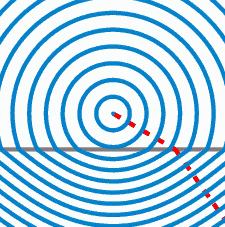
\includegraphics[width=150px]{Immagini/Snells_law_wavefronts.png}
    \captionsetup{width=.8\linewidth}
    \caption[\textit{By Oleg Alexandrov}]{\textit{By Oleg Alexandrov\footnotemark} Rappresentazione della deformazione subita da un'onda sferica al passaggio da un mezzo a indice di rifrazione minore ad uno con indice di rifrazione maggiore. La linea rossa, normale al fronte d'onda, evidenzia la rifrazione}
    \label{fig:wawefrontRefraction}
\end{figure}
\footnotetext{By Oleg Alexandrov, Public Domain, \href{https://commons.wikimedia.org/w/index.php?curid=3323373}{https://commons.wikimedia.org/w/index.php?curid=3323373}}

Il rallentamento della luce in in mezzo a maggiore densità non è dovuto a fenomeni di scattering o assorbimento, ma all'eccitazione degli elettroni del mezzo stesso che agiscono come un induttore. Questi infatti, stimolati dalla carica elettrica dei fotoni, iniziano a loro volta ad oscillare, producendo onde elettromagnetiche che fanno interferenza con l'onda di onde luminosa, producendo un'onda con frequenza minore\cite{Fermilab2019}.

\subsection{Derivazione della Legge di Snell dal Principio di Fermat}

La legge di Snell può essere derivata utilizzando il principio di Fermat, che afferma che il percorso seguito dalla luce tra due punti è quello che richiede il tempo minimo.

Consideriamo un raggio di luce, perpendicolare al fronte d'onda, che passa da un mezzo con indice di rifrazione \( n_1 \) a un altro mezzo con indice di rifrazione \( n_2 \) come in \cref{fig:snellsLaw}. Supponiamo che il raggio inizi nel punto \( Q \) nel primo mezzo e termini nel punto \( P \) nel secondo mezzo.

\begin{figure}[!ht]
    \centering
    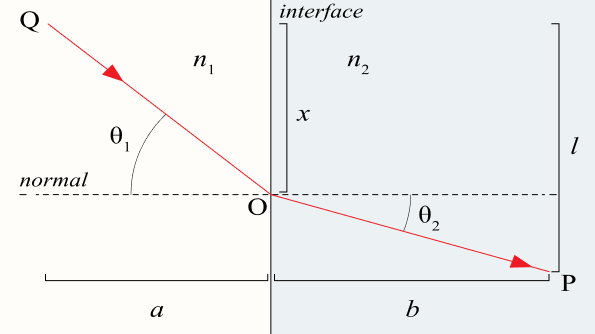
\includegraphics[width=\linewidth]{Immagini/Snells_law_Diagram_B_vector.png}
    \captionsetup{width=.8\linewidth}
    \caption[\textit{By Oleg Alexandrov}]{\textit{By Smedlib\footnotemark} Rappresentazione di un raggio luminoso al passaggio da un mezzo con indice di rifrazione minore \( n_1 \) ad uno con indice di rifrazione maggiore \( n_2 \)}
    \label{fig:snellsLaw}
\end{figure}
\footnotetext{By Smedlib, CC BY-SA 4.0, \href{https://commons.wikimedia.org/w/index.php?curid=60639100}{https://commons.wikimedia.org/w/index.php?curid=60639100}}


Il tempo impiegato dalla luce per percorrere il tratto \( Q \to O \to P \), dove \( O \) è il punto di incidenza sulla superficie di separazione, è dato da:

\[ t = \frac{QO}{v_1} + \frac{OP}{v_2} \]

dove \( v_1 \) e \( v_2 \) sono le velocità della luce nei rispettivi mezzi. Poiché la velocità della luce in un mezzo è inversamente proporzionale all'indice di rifrazione \( v_i = \frac{c}{n_i} \), possiamo riscrivere il tempo totale come:

\[ t = \frac{\sqrt{x^2 + a^2}}{v_1} + \frac{\sqrt{(l - x)^2 + b^2}}{v_2} \]
\[ t = \frac{\sqrt{x^2 + a^2} \, n_1}{c} + \frac{\sqrt{(l - x)^2 + b^2} \, n_2}{c} \]

Per trovare il tempo minimo deriviamo rispetto a \( x \):

\[ \frac{d}{dx} \left( \frac{\sqrt{x^2 + a^2} \, n_1}{c} + \frac{\sqrt{(l - x)^2 + b^2} \, n_2}{c} \right) = 0 \]

\[ \frac{n_1 x}{c \sqrt{x^2 + a^2}} - \frac{n_2 (l - x)}{c \sqrt{(l - x)^2 + b^2}} = 0 \]

Semblificando  \( c \) otteniamo:

\[ \frac{n_1 x}{\sqrt{x^2 + a^2}} = \frac{n_2 (l - x)}{\sqrt{(l - x)^2 + b^2}} \]

Riconoscendo che il seno degli angoli di incidenza (\( \theta_1 \)) e di rifrazione (\( \theta_2 \)) è rispettivamente dato da:

\[ \sin \theta_1 = \frac{x}{\sqrt{x^2 + a^2}} \]
\[ \sin \theta_2 = \frac{l - x}{\sqrt{(l - x)^2 + b^2}} \]

Possiamo scrivere:

\[ n_1 \sin \theta_1 = n_2 \sin \theta_2 \]

\section{Interferenza: L'Esperimento di Young}

\subsection{Descrizione dell'esperimento di Young}

L'esperimento di interferenza di Thomas Young, condotto nel 1801, è uno dei più celebri nella storia della fisica. Questo esperimento dimostrò la natura ondulatoria della luce e fu cruciale per la comprensione del fenomeno dell'interferenza. Nell'esperimento, Young fece entrare la luce solare in una stanza buia attraverso un foglio di carta spessa appositamente forato con un ago, in modo da ottenere un fascio luminoso orizzontale e sufficientemente collimato. Il raggio così ottenuto andava a proiettarsi sulla parete opposta a quella su cui si trovava la finestra da cui era entrato, sulla quale era possibile riscontrare gli effetti dell'interferenza.

Lungo il percorso del fascio di luce, ad una distanza nota dalla parete, era posto un ostacolo in grado di dividere il raggio in due. Nonostante sia passato alla storia come esperimento della doppia fenditura, nella prima versione Young aveva utilizzato una carta dello spessore di qualche decimo di millimetro. Il raggio, così diviso, andava a formare sulla parete una figura d'interferenza, che scompariva coprendone una delle due metà. Questo dimostrava che la figura di interferenza era dovuta all'interazione tra le due metà del fascio luminoso e non provocata dall'ostacolo.

La semplicità di questo esperimento e la sua rilevanza storica lo rendono ideale per la riproduzione da parte degli studenti, anche in mancanza di laboratori universitari. Sostituendo la luce solare con quella di un comune laser tascabile infatti, l'esperimento di Young è stato proposto nelle classi di liceo\cite{Scheider1986}. Con le restrizioni dovute alla pandemia scatenata dal SARS-CoV-2, che hanno imposto lo svolgimento delle lezioni in remoto, l'esperimento di Young è stato anche proposto agli studenti dell'università di Bologna come attività da svolgere direttamente a casa propria, utilizzando un CD come reticolo di diffrazione\cite{Campari2021}. 

\begin{figure}[!ht]
    \centering
    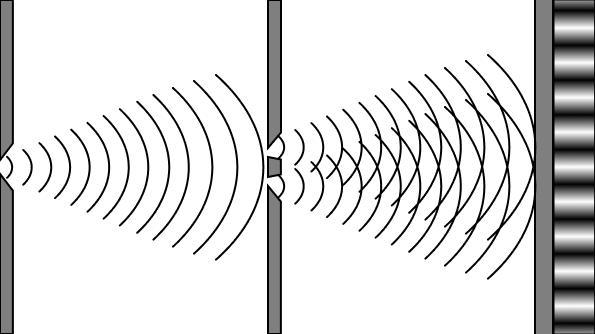
\includegraphics[width=\linewidth]{Immagini/double_slit_above.png}
    \captionsetup{width=.8\linewidth}
    \caption{Raffigurazione dell'esperimento della doppia fenditura.}
    \label{fig:doubleSlitAbove}
\end{figure}

In \cref{fig:doubleSlitAbove} è raffigurata la versione dell'esperimento che utilizza una doppia fenditura per separare il fascio luminoso. La trattazione numerica è identica, in quanto l'effetto di intereferenza è dato dalla differenza di cammino ottico \( \Delta r \) tra i due raggi e non dall'interazione con l'ostacolo, ma la rappresentazione risulta più chiara. Perciò sarà utilizzata questa versione per ricavare la posizione dei massimi e dei minimi di interferenza.

\subsection{Posizione dei massimi e dei minimi di interferenza}

Per trovare la posizione delle bande luminose (massimi di interferenza) e le zone buie (minimi di interfereza) nell'esperimento della doppia fenditura, consideriamo un'onda luminosa coerente (proveniente ad esempio da un laser) e monocromatica, la quale incide su una barriera con due fenditure separate da una distanza \(d\). 

La luce che passa attraverso le fenditure crea un pattern di interferenza su uno schermo situato a una distanza \(L\) dalle fenditure, con \(L \gg d \), in modo tale che i raggi \(r_1\) ed \(r_2\), che partono dalle due fessure e finiscono nello stesso punto sulla parete, possano essere considerati come paralleli.

\begin{figure}[!ht]
    \centering
    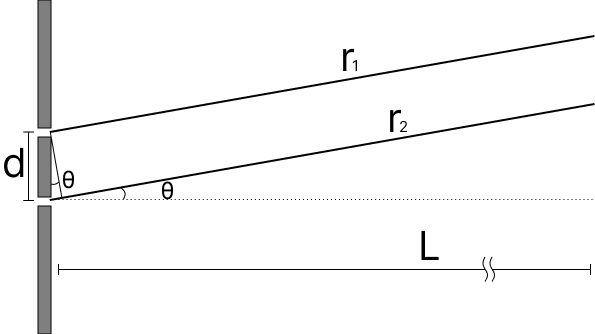
\includegraphics[width=\linewidth]{Immagini/double_slit_setup.png}
    \captionsetup{width=.8\linewidth}
    \caption{raffigurazione dell'esperimento della doppia fenditura visto dall'alto. Il fascio luminoso coerente originato da \d viene diviso in due }
    \label{fig:doubleSlitSetup}
\end{figure}

Da \cref{doubleSlitSetup} è anche facile vedere che l'angolo \(\theta\) di inclinazione dei raggi uscenti dalle fenditure è uguale all'angolo acuto del triangolo rettangolo che ha come ipotenusa \(O_1, O_2 \).

Questo comporta che la differenza di cammino ottico tra le due onde sia data da:

\[ \Delta L = d \sin \theta \]

dove \(\theta\) è l'angolo di deviazione della luce rispetto alla perpendicolare alle fenditure.

I massimi di interferenza si verificano quando la differenza di cammino ottico è un multiplo intero della lunghezza d'onda \(\lambda\):
 
\[ d \sin \theta = m \lambda \]

dove \(m\) (\(m = 0, \pm 1, \pm 2, \ldots\)) viene detto "ordine" del massimo di interferenza.
  
I minimi di interferenza si verificano quando la differenza di cammino ottico è un multiplo, dispari, di metà lunghezza d'onda: 

\[ d \sin \theta = \left( m + \frac{1}{2} \right) \lambda \]

Per \(\theta\) piccoli, possiamo approssimare \(\sin \theta \approx \tan \theta\). Se \(y\) è la distanza verticale dalla frangia centrale (frangia di ordine \(m=0\)) sullo schermo, allora:

\[ \tan \theta \approx \sin \theta \approx \frac{y}{L} \]

Sostituendo nella condizione per i massimi di interferenza:

\[ d \frac{y}{L} = m \lambda \]

Da cui la posizione delle frange di ordine \(m\) è:

\[ y = \frac{m \lambda L}{d} \]

Sostituendo nella condizione per i minimi di interferenza:

\[ d \frac{y}{L} = \left( m + \frac{1}{2} \right) \lambda \]

Da cui la posizione delle ombre di ordine \(m\) è:

\[ y = \frac{m + \frac{1}{2} \lambda L}{d} \]

\subsection{Importanza dell'interferenza nella spettroscopia}

L'interferenza è alla base di molte tecniche spettroscopiche avanzate. Ad esempio:

\begin{itemize}
\item \textbf{Spettroscopia a interferometria di Fourier (FTIR)}: Utilizza l'interferenza della luce per ottenere spettri con alta risoluzione e sensibilità. Un interferometro di Michelson è spesso utilizzato per dividere e ricombinare la luce, creando un interferogramma che viene successivamente trasformato in uno spettro utilizzando la trasformata di Fourier.
\item \textbf{Spettroscopia di diffrazione}: Utilizza reticelle di diffrazione per separare la luce in lunghezze d'onda componenti attraverso l'interferenza. Questo metodo è essenziale per l'analisi spettrale dettagliata in molteplici applicazioni scientifiche.
\item \textbf{Interferometria di Fabry-Perot}: Utilizza cavità risonanti per produrre frange di interferenza ad alta risoluzione, permettendo misurazioni precise delle lunghezze d'onda e delle frequenze della luce.
\end{itemize}

Queste tecniche dimostrano come il fenomeno dell'interferenza sia sfruttato in spettroscopia per analizzare la luce con estrema precisione, fornendo informazioni dettagliate sulla struttura e la composizione dei materiali \cite{born1999principles}.

\section{Emissione e Assorbimento di Radiazione: Il Modello Atomico di Bohr}

\subsection{Introduzione al modello atomico di Bohr}

Il modello atomico di Bohr, proposto da Niels Bohr nel 1913, rappresenta un punto di svolta nella comprensione della struttura atomica e dei processi di emissione e assorbimento della luce. Bohr introdusse l'idea che gli elettroni negli atomi orbitano intorno al nucleo in livelli di energia quantizzati, ovvero, gli elettroni possono occupare solo determinate orbite stazionarie con energie specifiche. Quando un elettrone salta da un'orbita a un'altra, assorbe o emette un fotone con energia pari alla differenza di energia tra le due orbite \cite{bohr1913constitution}.

\subsection{Spettri di emissione e assorbimento}

Gli spettri di emissione e assorbimento forniscono informazioni cruciali sulla struttura degli atomi e delle molecole.

\begin{itemize}
\item \textbf{Spettri di emissione}: Si osservano quando gli elettroni eccitati in un atomo o una molecola tornano a uno stato energetico inferiore, emettendo fotoni. Ogni elemento chimico ha uno spettro di emissione caratteristico, costituito da una serie di linee spettrali a lunghezze d'onda specifiche. Queste linee corrispondono alle transizioni energetiche degli elettroni tra i diversi livelli quantizzati.
\item \textbf{Spettri di assorbimento}: Si formano quando la luce bianca passa attraverso un gas o un liquido, e alcuni fotoni vengono assorbiti dagli atomi o dalle molecole del campione, portando gli elettroni a livelli energetici superiori. Le lunghezze d'onda assorbite appaiono come linee scure nello spettro continuo, corrispondenti alle stesse transizioni osservate negli spettri di emissione.
\end{itemize}

L'analisi degli spettri di emissione e assorbimento permette di identificare la composizione elementare di un campione e di studiare le proprietà fisiche e chimiche delle sostanze.

\subsection{Applicazioni e implicazioni nella spettroscopia}

Il modello atomico di Bohr ha avuto un impatto profondo sulla spettroscopia, fornendo una base teorica per comprendere i processi di emissione e assorbimento della radiazione elettromagnetica. Alcune delle applicazioni chiave includono:

\begin{itemize}
\item \textbf{Analisi chimica}: La spettroscopia di emissione e assorbimento è utilizzata per identificare gli elementi presenti in un campione, come nella spettroscopia di emissione atomica e nell'assorbimento atomico.
\item \textbf{Astrofisica}: Gli spettri di emissione e assorbimento delle stelle e di altri corpi celesti forniscono informazioni sulla loro composizione chimica, temperatura e densità.
\item \textbf{Diagnostica medica}: Tecniche spettroscopiche basate sull'emissione e l'assorbimento sono utilizzate per analizzare campioni biologici, come nella spettroscopia a fluorescenza per la rilevazione di biomarcatori.
\end{itemize}

L'approccio quantistico introdotto da Bohr è stato ulteriormente sviluppato dalla meccanica quantistica moderna, che ha raffinato la comprensione delle interazioni tra luce e materia, consentendo tecniche spettroscopiche sempre più precise e avanzate.

\section{Risultati Principali della Spettroscopia}

\subsection{Identificazione degli elementi e delle molecole}

La spettroscopia è uno strumento fondamentale per l'identificazione degli elementi chimici e delle molecole. Ogni elemento emette o assorbe radiazione a lunghezze d'onda specifiche, creando uno spettro unico che funge da "impronta digitale" caratteristica. Questo permette di determinare la composizione elementare di campioni sconosciuti. Ad esempio, nella spettroscopia di emissione atomica, l'analisi delle linee spettrali emesse da un campione permette di identificare gli elementi presenti. Analogamente, nella spettroscopia di assorbimento, le lunghezze d'onda assorbite indicano la presenza di specifici elementi o molecole nel campione \cite{strasburger2014spectroscopy}.

\subsection{Analisi della composizione chimica delle stelle}

In astrofisica, la spettroscopia è uno strumento cruciale per studiare la composizione chimica delle stelle e di altri corpi celesti. Analizzando gli spettri di emissione e assorbimento delle stelle, gli scienziati possono determinare gli elementi presenti nelle loro atmosfere. Questa tecnica, nota come spettroscopia stellare, ha permesso di scoprire che le stelle sono composte principalmente da idrogeno ed elio, con tracce di altri elementi. Inoltre, la spettroscopia permette di studiare le condizioni fisiche delle stelle, come la temperatura e la densità, fornendo informazioni preziose sulla loro evoluzione e sulla struttura dell'universo.

\subsection{Applicazioni nella medicina e nella biologia}

La spettroscopia ha numerose applicazioni in medicina e biologia. In medicina, è utilizzata per la diagnosi e il monitoraggio di diverse condizioni cliniche. Ad esempio, la spettroscopia di risonanza magnetica nucleare (NMR) è impiegata per ottenere immagini dettagliate del corpo umano, permettendo la diagnosi di tumori e altre patologie. La spettroscopia a fluorescenza è utilizzata per rilevare biomarcatori e monitorare processi biologici in tempo reale. In biologia, la spettroscopia infrarossa e la spettroscopia Raman sono utilizzate per studiare le strutture molecolari e le interazioni nelle cellule e nei tessuti, fornendo informazioni fondamentali sulla biochimica e sulla fisiologia.

La capacità della spettroscopia di fornire informazioni dettagliate sulla composizione chimica e sulle proprietà fisiche dei campioni la rende uno strumento indispensabile in molteplici campi scientifici e applicativi. Le sue applicazioni spaziano dalla ricerca fondamentale alla diagnostica clinica, dimostrando la versatilità e l'importanza di questa tecnica.

\section{Tecniche Avanzate di Spettroscopia}

\subsection{Spettroscopia a trasformata di Fourier (FTIR)}

La spettroscopia a trasformata di Fourier (FTIR) è una tecnica potente che sfrutta l'interferometria per ottenere spettri con alta risoluzione e sensibilità. In un interferometro di Michelson, un raggio di luce viene diviso in due percorsi che vengono poi ricombinati, producendo un interferogramma. Questo interferogramma contiene tutte le informazioni spettrali del campione e viene trasformato in uno spettro attraverso la trasformata di Fourier. L'FTIR è particolarmente utile per analizzare campioni complessi, come miscele chimiche, perché permette di identificare e quantificare i componenti in modo rapido e preciso \cite{griffiths2007fourier}.

\subsection{Spettroscopia Raman}

La spettroscopia Raman è una tecnica non distruttiva che si basa sulla diffusione inelastica della luce. Quando la luce interagisce con una molecola, la maggior parte della luce viene diffusa elasticamente (effetto Rayleigh), ma una piccola frazione viene diffusa inelasticamente, con un cambiamento in energia corrispondente alle vibrazioni molecolari. Questo cambiamento energetico produce uno spettro Raman caratteristico che può essere utilizzato per identificare le molecole e studiare le loro interazioni. La spettroscopia Raman è ampiamente utilizzata in chimica, fisica, biologia e scienze dei materiali per analizzare la composizione molecolare e strutturale dei campioni.

\subsection{Spettroscopia di risonanza magnetica nucleare (NMR)}

La spettroscopia di risonanza magnetica nucleare (NMR) è una tecnica estremamente potente per lo studio della struttura molecolare. Basata sull'interazione tra i nuclei atomici e un campo magnetico esterno, l'NMR fornisce informazioni dettagliate sulla disposizione degli atomi in una molecola. Quando i nuclei atomici, come quelli dell'idrogeno o del carbonio-13, sono immersi in un campo magnetico e irradiati con onde radio, assorbono energia e poi la rilasciano, producendo un segnale caratteristico. Questo segnale può essere analizzato per determinare la struttura chimica e conformazionale delle molecole. L'NMR è particolarmente utile in chimica organica e biochimica per identificare e caratterizzare composti organici e biomolecole.

\subsection{Altre tecniche spettroscopiche avanzate}

Oltre a FTIR, Raman e NMR, esistono numerose altre tecniche spettroscopiche avanzate, ciascuna con applicazioni specifiche:

\begin{itemize}
\item \textbf{Spettroscopia XPS (X-ray Photoelectron Spectroscopy)}: Utilizzata per studiare la composizione elementare e lo stato chimico delle superfici.
\item \textbf{Spettroscopia EPR (Electron Paramagnetic Resonance)}: Impiegata per analizzare specie con elettroni spaiati, come radicali liberi e centri di metalli di transizione.
\item \textbf{Spettroscopia di massa ad alta risoluzione (HRMS)}: Fornisce informazioni dettagliate sulla massa e la struttura dei composti chimici, utile per analisi precise e identificazione di molecole complesse.
\end{itemize}

Queste tecniche avanzate di spettroscopia permettono di ottenere una comprensione approfondita delle proprietà chimiche e fisiche dei materiali, aprendo nuove frontiere nella ricerca scientifica e nelle applicazioni tecnologiche.

\section{Conclusioni e Prospettive Future}

\subsection{Riepilogo dei punti chiave}

La spettroscopia rappresenta una delle tecniche più versatili e potenti nella scienza moderna, permettendo di studiare l'interazione tra la luce e la materia per ottenere informazioni dettagliate sulla composizione, struttura e dinamica dei materiali. Attraverso principi fondamentali come la rifrazione (illustrata dalla Legge di Snell) e l'interferenza (dimostrata dall'esperimento di Young), e grazie a modelli teorici come quello atomico di Bohr, la spettroscopia ha fornito strumenti essenziali per l'identificazione e l'analisi di elementi e molecole.

Tecniche avanzate come la spettroscopia a trasformata di Fourier (FTIR), la spettroscopia Raman e la risonanza magnetica nucleare (NMR) hanno ampliato ulteriormente le possibilità di questa disciplina, permettendo applicazioni che vanno dalla chimica all'astrofisica, dalla biologia alla medicina. Questi sviluppi hanno rivoluzionato il modo in cui comprendiamo la materia e le sue interazioni, portando a scoperte fondamentali e innovazioni tecnologiche.

\subsection{Sviluppi recenti e future direzioni della ricerca spettroscopica}

La ricerca spettroscopica è in continua evoluzione, guidata dalla necessità di migliorare la risoluzione, la sensibilità e la velocità delle tecniche esistenti, nonché di sviluppare nuove metodologie per affrontare sfide scientifiche emergenti. Alcuni dei principali sviluppi recenti e delle prospettive future includono:

\begin{itemize}
\item \textbf{Spettroscopia ultrarapida}: Tecniche che utilizzano impulsi laser femtosecondi per studiare processi dinamici ultra veloci in molecole e materiali. Queste tecniche permettono di osservare reazioni chimiche e transizioni di fase in tempo reale, aprendo nuove possibilità nella chimica e nella fisica dei materiali.
\item \textbf{Spettroscopia a singola molecola}: Permette di studiare le proprietà e le dinamiche di singole molecole, fornendo una visione dettagliata delle interazioni molecolari e dei processi biologici a un livello senza precedenti. Questa tecnica ha applicazioni in biologia, chimica e scienze dei materiali.
\item \textbf{Spettroscopia di imaging}: Combina la spettroscopia con tecniche di imaging per ottenere mappe spaziali dettagliate delle proprietà chimiche e fisiche dei campioni. Questo approccio è particolarmente utile in scienze dei materiali, biologia e medicina per studiare la distribuzione di elementi e composti in campioni complessi.
\item \textbf{Intelligenza artificiale e apprendimento automatico}: L'uso di algoritmi di intelligenza artificiale per analizzare grandi dataset spettroscopici sta rivoluzionando il modo in cui vengono interpretati i dati, permettendo analisi più rapide e accurate e la scoperta di nuove correlazioni e fenomeni.
\item \textbf{Spettroscopia in ambienti estremi}: Lo sviluppo di tecniche spettroscopiche per studiare materiali e processi in condizioni estreme di temperatura, pressione e campo magnetico, è essenziale per la ricerca in fisica dei materiali e geoscienze.
\end{itemize}

Questi sviluppi promettono di espandere ulteriormente le applicazioni della spettroscopia, offrendo nuove opportunità per la ricerca scientifica e l'innovazione tecnologica. La spettroscopia continuerà a giocare un ruolo cruciale nella comprensione e nell'ingegnerizzazione del mondo naturale, contribuendo al progresso in molti campi della scienza e della tecnologia \cite{johnson2020future}.

\chapter{Il mio lavoro}
\section{Modalità di Redazione e Gestione dei Contenuti}
\subsection{Il processo di creazione e modifica delle voci}
\subsection{Regole e linee guida per i contributori}
\subsection{Il ruolo dei revisori e degli amministratori}
\subsection{Strumenti e tecnologie utilizzati}

\newpage

\printbibliography


\end{document}

